\section{Multi-weight} \label{sec:intro}


\begin{table}
\begin{tabular*}{\columnwidth}{|l|p{0.76\columnwidth}|}
\hline
\bf Symbol		& \bf Meaning \\\hline
$G\mathbf{(V,E)}$ 	& A graph with node set $V$ and edge set $E$ \\\hline 
$v_i$			& A node in $V$ \\\hline 
$(v_i,v_j)$		& An edge in $E$ \\\hline 
$\omega_k(v_i,v_j)$	& The edge weight of $(v_i,v_j)$ using weight category $\varsigma_k \in \mathcal{W}$ \\\hline
$\mathcal{W}$		& Set of possible weight categories $\mathcal{W}$, where $\varsigma_k$ denotes the category $k$ \\\hline

$Q_{s,t,w}$		& \spath query from node $v_s$ to node $v_t$, using weight $w$\\\hline
$P_{s,t,w}$		& The \spath result of $Q_{s,t,w}$ \\\hline
$|P_{s,t,w}|$		& The size of $P_{s,t,w}$ (in number of nodes) \\\hline
$E_{s,t,w}$		& The expense of executing query $Q_{s,t,w}$ \\\hline
$\chi_{s,t,w}$		& The frequency of a \spath with weight type w \\\hline
$\Psi$ 			& The Cache \\\hline
$\mathfrak{U}_w(P_{s,t,w})$& The set of all subpaths in $P_{s,t,w}$ \\\hline
$\mathfrak{U}_w(\Psi)$	& The set of all subpaths of paths in $\Psi$ \\\hline
$\gamma_w(\Psi)$		& The total benefit of the content in the cache \\\hline

$d_{s,t,w}$		& The \spath distance of a path $P_{s,t,w}$ \\\hline
$\mathcal{QL}$		& Query log of search queries \\\hline
\end{tabular*}
\caption{Table of Symbols \textbf{MW}}
\label{tab:symbols}
\end{table}

% 
% 
% \begin{algorithm}[bht]
% \dontprintsemicolon
% \SetVline
% 
% \SetKwInOut{Input}{input}\SetKwInOut{Output}{output}\SetKw{Return}{return}
% 
% \Input{
% 
% 	$(q,R)$: A Range query\;
% 	$\mathcal{O}$: A set of POI \;
% }
% 
% \Output{
% 
% 	A set \poi $\in \mathcal{O}$ \;
% }
% 
% \funcc{Fair}{(q,R), \mathcal{O}}
% {
%     \ForEach{$o_i \in \mathcal{O} : \mathfrak{d}_{q,o_i} \leq R$}
%     {
%       $candidate_{\mathcal{O}} \leftarrow o_i$ \;
%     }
%     result $\leftarrow$ \naivens((q,R), $candidate_{\mathcal{O}}$) \;
% 
%     \Return{result} \;
% }
% 
% \caption{Fair Algorithm}
% \label{alg:fair}
% \end{algorithm}


In multi-weight road networks\cite{icdeMouratidisLY10} a shortest path queries may be submitted to a service provider based on different shortest path metrics or categories. A metric could be the fastest route, the fewest number of edges to traverse, or of casue the actual shortest distance. These kind of queries require the \spath service provider to have several weights defined for each edge, a fair assumption on most service providers (TODO: CITE).
Such queries precent a challange to effectively cache, as the same \spath $P_{s,t,w}$ may not be valid for all weights/metrics $w$.




\begin{definition}
Let $G(V, E)$ be a graph with a set $V$ of nodes and a set $E$ of edges.
Each node $v_i \in V$ models a road junction. Each edge $(v_i, v_j) \in
E$ models a road segment. The weight (length) of an edge is denoted as $W(v_i, v_j, w)$, where $w \in \mathcal{W}$ is the weight type (length, travel time, scenic value, ect.).
\end{definition}



\begin{definition}{Multi-weight Search}\\
A Multi-weight Search query, denoted by $Q_{s,t,w}$ consist of a source and target vertex $s$ and $t$, plus a weight type $w \in \mathcal{W}$ 
The result of $Q_{s,t,w}$, denoted $SP_{s,t,w}$, is a collection of connected vertices $v_s,\dotsc,v_t$ such that they form a \spath on graph $G\mathbf{(V,E)}$ using weight-type $w \in \mathcal{W}$.
\end{definition}


Using the map in figure \ref{fig:map1} a multi-weight search query, $Q_{v_1,v_2,w}$, can be executed for two different weights, $w_1$ or $w_2$, possibly resulting in two different paths for the same start-/end-nodes, depending on the weight chosen. Table \ref{tab:expsi} shows the \spath $\psi_1$ and $\psi_2$ resulting from the same start-/end-node, but using different weights ($w_1, w_2$).


\begin{definition}{Multi-weight Query Log ($\mathcal{QL_W}$)}\\
A multi-weight search query log $\mathcal{QL_W}$ is a collection of time stamped queries that have been issued by users in the past.
A query is on the form $(s,t,w)$, where $s$ and $t$ is the start- and end-point respectively. $W$ is the weight type to be used when calculating the SP. The full form of the log, $\mathcal{QL_W}$,  is then: $\{(s_0,t_0,w_0),\dots,(s_i,t_i,w_i)\}$. $\chi_{s,t}$ will be the number of sub paths seen, regardless of their weight type, the cost table for $E_{s,t}$ will however need to be maintained for each individual weight type, as each type can incur a different SP.
\end{definition}


\begin{figure}[hbt]
  \center
        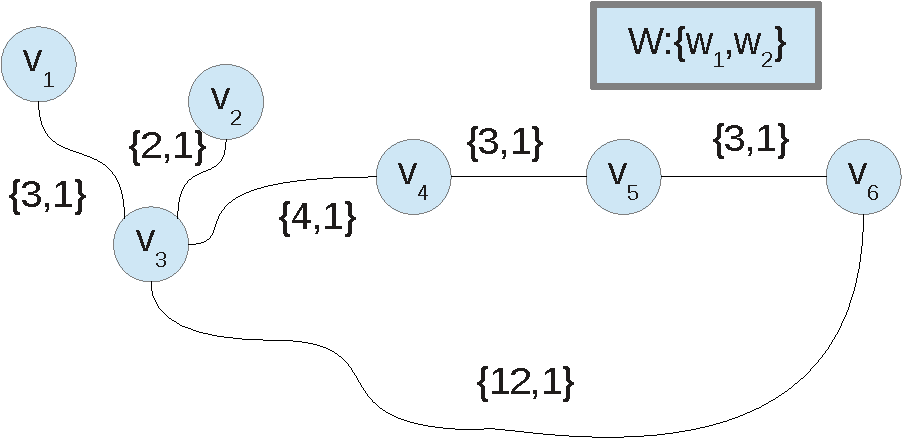
\includegraphics[width=0.4\textwidth]{figures/map1}
        \caption{Map of fig \ref{fig:wilist} and table \ref{tab:expsi}, with set of weights on the edges}
  \label{fig:map1}
\end{figure}


\subsection{Cache Structure}

Paths stored as they are in the cache. Instead of using a single inverted list to look up whether the cache can answer a query, we use a collection of inverted lists to keep track of which $Q_{s,t,w}$ can be answered by the cache $\Psi$, for each weight type in $\mathcal{W}$.
Even if a full path can only answer a query for a single weight type, then by using this approach then any sub-path able to answer for more than one weight-type will still be utilized. 

As a path that can answer a SP query for more than one weight type is more valuable then we maintain $\chi_{s,t,\_}$ without regards to the weight type, simply adding up the statistics for each query, for all weight types seen. (This does however not necessarily work very well when we calculate $\chi_{R_i,R_j,w}$ for a pair of regions). 

The map in  fig \ref{fig:map1} depicts a simple road system with 2 different weights on each edge. The first edge weight captures edge length, while the second weight captures the of number of edges traversed, which is why each edge always contributes 1.

Using two example queries, $Q_{v1,v6,\_}, Q_{v1,v5,\_}$, on the map in figure \ref{fig:map1}, we will get the cache items in table \ref{tab:expsi}. Using this we build a inverted list for each weight in order to quickly answer queries (see fig. \ref{fig:wilist}). 
To answer a query $Q_{v_s,v_t,w}$ we use $w$ to first find the relevant inverted list. Afterwards we do 2 look-ups in the inverted list, for $v_s$ \& $v_t$, and do the intersection of the resulting cache items. If the answer is non-empty there is a \spath for $Q_{v_s,v_t,w}$ in the cache.

The same query with different weight can result in different cache items. In table \ref{tab:expsi} the query $Q_{v_1,v_6,X}$ ($X: w_1,w_2$) results in both $\psi_1$ and $\psi_2$ being added to the cache, since the query returns two different paths for weights $w_1$ and $w_2$. It might of cause also be the case that no matter what weight we use, then the \spath is the same. $Q_{v_1,v_5,X}$ show this well, as the \spath does not change for the two weights. One important aspect to notice is that if a full cache item is only valid for a single weight, but a sub path of the \spath is valid for several weights, then this fact will captured in the inverted lists, maximizing the reuse of items in the cache, making them more useful. 



\subsection{Benefit Model}

We extend the benefit driven benefit model introduced in \cite{thomsen2012}. We introduce what changes are needed to capture the benefit of \spaths with \textit{multi-weight search}.
Equation \ref{eq:phiw}, \ref{eq:upsw}, \ref{eq:benefitw}, and \ref{eq:cachebenefitw} define the existing functions with restriction on $w$.


We have to answer two important questions:
\begin{enumerate}
\item \label{quest:impone} Which queries $Q_{s,t,w}$ can be answered by the path $P_{s,t,w}$?
\item \label{quest:imptwo} For query $Q_{s,t,w}$ what is the benefit if added to the cache.
\end{enumerate}

Question \ref{quest:impone} can be answered by the updated lemma \ref{lem:weightedoptimalproperty} (from \cite{thomsen2012}). A path $P_{a,b,d}$ contains the path $P_{s,t,w}$ if they share the same weight and both $v_s$ \& $v_t$ are on $P_{a,b,d}$. With this we get the updated definition for the \textit{answerable query set}, $\mathfrak{U}_w(P_{a,b,d})$, for path $P_{a,b,d}$:

\begin{equation} \label{eq:phiw}
\mathfrak{U}_w(P_{a,b,d}) = \{ P_{s,t,w} : s, t \in P_{a,b,d},  s \neq t,  d = w\}
\end{equation}

Equation \ref{eq:phiw} finds all sub-paths of SP $sp$ with weight category $w$. Using cache item $\psi_1$ from $Q_{v_1,v_6}$ in table \ref{tab:expsi}, the answerable queryset is: $\mathfrak{U}_w(P_{1,6,w_1}) = \{P_{1,3,w_1},P_{1,4,w_1},P_{1,5,w_1},P_{1,6,w_1},P_{3,4,w_1},$ $P_{3,5,w_1},P_{3,6,w_1},P_{4,5,w_1},P_{4,6,w_1},P_{5,6,w_1}\}$ 


\begin{table}
\begin{tabular}{l|l|l}\hline
$\psi$		& Cache item 			& Weight category \\\hline  \hline
$\psi_1:$	& $\{v_1,v_3,v_4,v_5,v_6\}$ 	& ($w_1$)\\\hline
$\psi_2:$	& $\{v_1,v_3,v_6\}$ 		& ($w_2$)\\\hline
$\psi_3:$	& $\{v_1,v_3,v_4,v_5\}$ 	& ($w_1,w_2$)\\\hline
\end{tabular}
\caption{Cache items using queries $Q_{v_1,v_6,X}, Q_{v_1,v_5,X}$ with $X:\{w_1,w_2\}$, covering both weights on the map (fig \ref{fig:map1})}
\label{tab:expsi}
\end{table}


In regards to question \ref{quest:imptwo} we update the \textit{benefit} equation $\gamma(\Psi)$ to consider weight categories:

\begin{equation} \label{eq:benefitw}
\gamma_w(P_{a,b,d}) = \sum\limits_{P_{s,t,w} \in \mathfrak{U}_w(P_{a,b,d})} \chi_{s,t,w} \bullet E_{s,t,w}
\end{equation}

Equation \ref{eq:benefitw} defines $benefit$ and makes it clear how much can we expect to save, in total, if path $P_{a,b,d}$ is in the cache. It is calculed based on the historical statistics defined by $\chi_{a,b,d}$ (equation \ref{eq:chiw}) and the cost of calculating the \spathns, $E_{a,b,d}$.


\begin{equation} \label{eq:chiw}
\chi_{s,t,w} =  |\{ Q_{b,e,w} \in \mathcal{QL}: s, t \in Q_{b,e,w} \}|
\end{equation}
Equation \ref{eq:chiw} defines the benefit of a path, based on how often we have seen the path, and its subpaths, in the query log $\mathcal{QL}$


\begin{lemma} \label{lem:weightedoptimalproperty}
\textbf{Weighted optimal subpath property} (modified from \cite{thomsen2012}, Lemma 1)\\

The \spath $P_{a,b,d}$ contain the \spath $P_{s,t,w}$ if $v_s \in P_{a,b,d}, v_t \in {P_a,b,d}$ and $d = w$, where $d,w \in \mathcal{W}$
Let $P_{a,b,d}$
Specifically, let $P_{a,b,d} = \langle v_{x_0},v_{x_1},v_{x_2},...,v_{x_m}\rangle$. 
We have $P_{s,t,w} = \langle v_{x_i},v_{x_i+1},...,v_{x_j}\rangle$ if $v_s = v_{x_i}, v_t = v_{x_j}$, and $w = d$ for some i,j such that $0 \leq i \leq j \leq m$
\end{lemma}



For the general case where the cache contains more than one path, the updated equations are shown below:


\begin{equation} \label{eq:phil}
\mathfrak{U}_l(P_{a,b,m})= \{ P_{s,t,l}: s,t \in P_{a,b,m}, s \neq t, m = l\}
\end{equation}


\begin{equation} \label{eq:upsw}
 \mathfrak{U}_w(\Psi) = \bigcup\limits_{P_{a,b,w} \in \Psi} \mathfrak{U}_w(P_{a,b,d})
\end{equation}

\begin{equation} \label{eq:cachebenefitw}
\gamma_w(\Psi) = \sum\limits_{P_{s,t,w} \in \mathfrak{U}_w(\Psi)} \chi_{s,t,w} \bullet E_{s,t,w}
\end{equation}

Equation \ref{eq:cachebenefitw} calculate the benefit of the cache with respect to a specific weight category, using $\chi_{s,t,w}$ and $E_{s,t,w}$, in the same way $\chi_{s,t}$ is calculated using $\chi_{s,t}$ and $E_{s,t}$.

Equation \ref{eq:upsw} finds the set of unique paths with weight $w$ from $\Psi$, which is either a path from $a$ to $b$, or a sub-path of such a path. This is the answerable set of paths using  $P_{a,b,d}$.




\begin{figure}[hbt]
  \center
        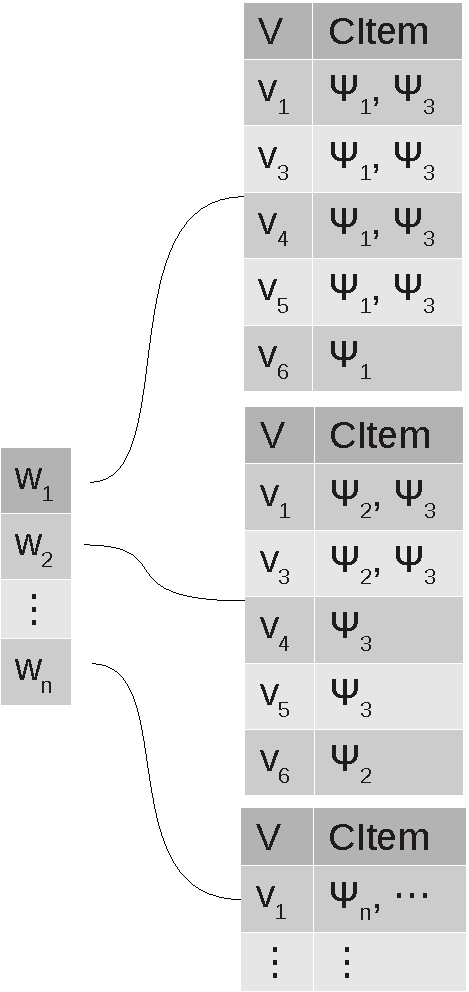
\includegraphics[width=0.25\textwidth]{figures/wilist}
        \caption{Cache structure for inverted lists using map from fig \ref{fig:map1} and cache elements from table \ref{tab:expsi}}
  \label{fig:wilist}
\end{figure}


% 
% \begin{tabular}{|l|l|}\hline
% \textbf{V} &	\textbf{Cache Item} \\\hline
% $V_1$	&	$\psi_1, \psi_3$ \\\hline
% $V_3$	&	$\psi_1, \psi_3$ \\\hline
% $V_4$	&	$\psi_1, \psi_3$ \\\hline
% $V_5$	&	$\psi_1, \psi_3$ \\\hline
% $V_6$	&	$\psi_1$ \\\hline
% \end{tabular}
% \vspace{2em}
% 
% \begin{tabular}{|l|l|}\hline
% \textbf{V} &	\textbf{Cache Item} \\\hline
% $V_1$	&	$\psi_2, \psi_3$ \\\hline
% $V_3$	&	$\psi_2, \psi_3$ \\\hline
% $V_4$	&	$\psi_3$ \\\hline
% $V_5$	&	$\psi_3$ \\\hline
% $V_6$	&	$\psi_2$ \\\hline
% \end{tabular}

\section{Direction Assistance}


\begin{table}
\begin{tabular*}{\columnwidth}{|l|p{0.76\columnwidth}|}
\hline
\bf Symbol		& \bf Meaning \\\hline
$G\mathbf{(V,E)}$ 	& A graph with node set $V$ and edge set $E$ \\\hline 
$v_i$			& A node in $V$ \\\hline 
$(v_i,v_j)$		& An edge in $E$ \\\hline 

$Q_{s,t,l}$		& \spath query from node $v_s$ to node $v_t$, using \textit{path level l}\\\hline
$P_{s,t,l}$		& The \spath result of $Q_{s,t,l}$, using \textit{path level l}. \\\hline
$|P_{s,t,l}|$		& The size of $P_{s,t,l}$ (in number of nodes) \\\hline
$E_{s,t,l}$		& The expense of executing query $Q_{s,t,l}$ \\\hline
$\chi_{s,t,l}$		& The frequency of a \spath with level $l$ \\\hline
$\Psi$ 			& The Cache \\\hline
$\mathfrak{U}_l(P_{s,t,l})$& The set of all subpaths in $P_{s,t,l}$ \\\hline
$\mathfrak{U}_l(\Psi)$	& The set of all subpaths of paths in $\Psi$ \\\hline
$\gamma_l(\Psi)$		& The total benefit of the content in the cache \\\hline

$d_{s,t,l}$		& The \spath distance of a path $P_{s,t,l}$ \\\hline

$\mathcal{QL}$		& Query log of search queries \\\hline
\end{tabular*}
\caption{Table of Symbols \textbf{DA}}
\label{tab:symbols}
\end{table}

When looking for directions to some place, a user who issues a \spath query does not actually care about the full \spathns\cite{sigmodTaoSP11}, but rather the user just wants to know when a new action is needed (turn left, right, or , besides following the current path. This is what GPS devices usually do. GPS devices usually only alerts the user if an action is needed, otherwise the user should just continue on the current path.
There are 2 overall levels that directions to follow a \spath can be given:

\begin{tabular}{@{}lp{21em} }
Finest 		& Level 1, the directions can be given for every single node on the \spathns, regardless of whether there are any option to change directions. \\
Coarsest	& Level 2, the directions can be given only when it is necessary to change directions, i.e. it does not matter how many side roads are passed, as long as the instruction is ostensibly "continue straight", then the instruction will not be included. Only if it is really necessary to make an action, such as turning, will the node be included in the instructions.
\end{tabular}

Both $finest$ and $coarsest$ will always include the start- and end-node. An alternative 'middleway' could be to have the directions be given only for nodes where it is possible to change direction/turn. 

When using $finest$ the advantage is that all subpaths of a \spath in the cache will be answerable, this scheme may however take op a lot of space for subpaths that are never seen, and therefor contribute no benefit to the cache.

Using $coarsest$ the advantage is that, especially on longer \spathsns, it will consume less space, while still maintaining enough information in the cache to be useful. The downside is of cause that the reduced number of vertices stored also negatively impacts the number of queries that can be answered by the \spath when it is in the cache.

In figure \ref{fig:minroute} a path from S to T is shown. Each vertex is enumerated based on what level of directions each node would be included in, according to the enumeration of \textit{finests} and \textit{coarsest} above


\begin{figure}[hbt]
  \center
        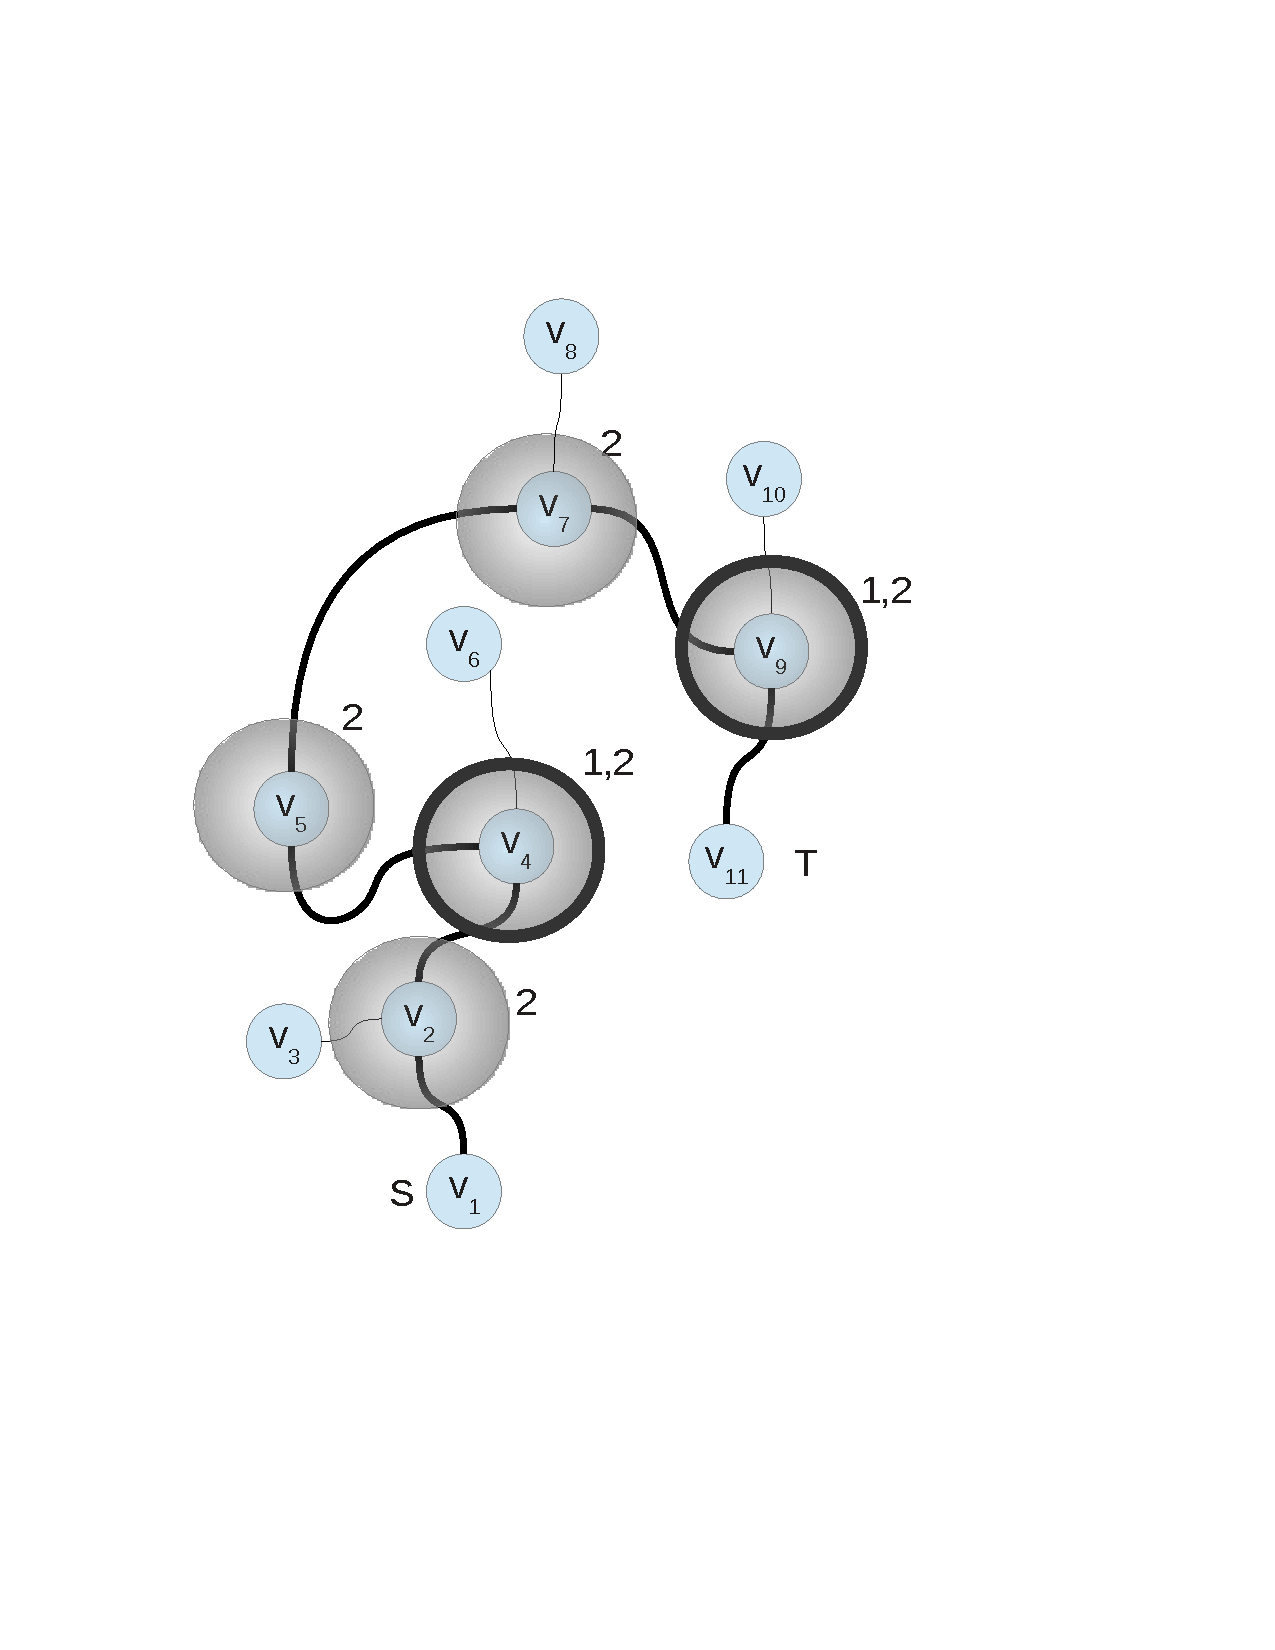
\includegraphics[width=0.4\textwidth]{figures/minroute}
        \caption{$Q_{1,11,l}$: Bold line from S to T denote travel route. $l$=Finest: All nodes on the path has a value 1, forming the complete path. 
        $l$=Coarsest: Circles with a value 2 denote the minimum set of nodes needed to navigate from S to T}
  \label{fig:minroute}
\end{figure}


\begin{definition}\label{def:direction} {Direction}\\
The \textit{directions} of a query $Q_{s,t,l}$, where the detail level $l$ is specified by 1(finest) or 2(coarsest), are a set of vertex neighbour pairs $\{(v_i,v_j),...\}$, each pair consisting of two connected nodes on $P_{s,t,l}$, representing a instruction at a node $v_i$, to take the path towards node $v_j$, where$v_i,v_j \in V$ on the \spath $P_{s,t,l}$.
\end{definition}

Figure \ref{fig:minroute} illustrates the $directions$ on query $Q_{1,11,l}$ for l being set to both coarsest and finest. For l=finest the $directions$ include the all vertices on the bold path from S to T. For l=coarsest the $directions$ only include the circled vertices: The start- and end-vertex plus a pair of neighbouring nodes each time the default action of going straight needs to be changed because the path turns where there are more than one choice.

\begin{definition}
Let $G(V, E)$ be a graph with a set $V$ of nodes and a set $E$ of edges.
Each node $v_i \in V$ models a road junction. Each edge $(v_i, v_j) \in
E$ models a road segment. The weight (length) of an edge is denoted as $W(v_i, v_j)$.
\end{definition}


\begin{definition}{\spathns: Query and Result}\\
A shortest path query, denoted by $Q_{s,t,l}$ consist of a source and target node, $v_s,v_t$.

The result of $Q_{s,t,l}$, denoted $P_{s,t,l}$, is a collection of nodes on the \spath from $v_s$ to $v_t$ (on the graph G) with each node associated with a direction (definition \ref{def:direction}).
We can represent $P_{s,t,l}$ as a list of pairs (node, neighbour node): $\langle (v_{x_0},v_{x_{0n}}), (v_{x_1},v_{x_{1n}}), \dots ,(v_{x_n},v_{x_{nn}}) \rangle$, where each pair contains a set of neighbouring virtices from $G$ level $l$ makes it necessary in order to provide the level of instruction asked for in $Q_{s,t,l}$.
\end{definition}




\subsection{Cache Structure}

Cache items can be stored just as they did before (\cite{thomsen2012}), either in a path array or as a graph representation. The main difference will be in the way the cache is accessed. Previously the key was simply the start and end node, and if they both had at least one common cache item then it was considered a cachehit (see figure 9 in \cite{thomsen2012}). Now the key will be a pair ($v_s, l$) and ($v_t, l$) for the start-/end-node. Table \ref{tab:directioninvlists} shows the inverted lists for different detail levels, based the cache content in table \ref{tab:psilvlcontent} and the map from figure \ref{fig:minroute}. Table \ref{tab:directioninvlists} shows the tables as three seperate tables, there is however no reason they could not be combined, so different keys ($v_i,l$) point to the same data.

Figuring out at what detail level paths should be stored in the cache, and whether the should be stored in a path array or as a graph representation is one of the interresting questions we want to answer. 

For longer \spaths that are relatively simple, meaning few instructions are needed, we will store very few nodes at level 3. This could be a problem as we have no information about how to traverse large parts of such a shortest path, even if such parts may be have high benefit (high $chi$ values for pairs of nodes on the path). We could possibly use the $\chi$ benefit values to determine how many extra vertices we have to store besides the ones at level 3. This would allow us to store only the nodes that are both necessary and useful for navigation.


\begin{table}
\begin{tabular}{@{}l@{}l@{}|@{}l@{}|@{}l@{}|@{}l@{}|@{}}\cline{3-5}
			&		& \bf l = 1				& \bf l = 2 			& \bf l = Alternative\\\cline{3-5}
$Q_{v_1,v_{11},l}$	& ($\Psi_1$)	& $v_1,v_2,v_4,v_5,v_7,v_8,v_9,v_{11}$ 	& $v_1,v_4,v_5,v_9,v_{11}$ 	& $v_1,v_2,v_4,v_5,v_9,v_{11}$\\\cline{3-5}
$Q_{v_3,v_8,l}$		& ($\Psi_2$)	& $v_3,v_2,v_4,v_5,v_7,v_8$		& $v_3,v_2,v_4,v_5,v_8$ 	& $v_3,v_2,v_4,_5,v_8$\\\cline{3-5}
$Q_{v_2,v_6,l}$		& ($\Psi_3$)	& $v_2,v_4,v_6$				& $v_2,v_6$			& $v_2,v_4,v_6$\\\cline{3-5}
\end{tabular}
  \caption{Example of how cache items will look when executed at different detail level}
  \label{tab:psilvlcontent}
\end{table}

\begin{table}
\begin{tabular}{c c c}
  \begin{tabular}{l|l|}\cline{2-2}
		  & \bf l = 1			 \\\cline{2-2}
  $v_1$		& $\Psi_1$			 \\\cline{2-2}
  $v_2$		& $\Psi_1,\Psi_2,\Psi_3$	 \\\cline{2-2}
  $v_3$		& $\Psi_2$			 \\\cline{2-2}
  $v_4$		& $\Psi_1,\Psi_2,\Psi_3$	 \\\cline{2-2}
  $v_5$		& $\Psi_1,\Psi_2$		 \\\cline{2-2}
  $v_6$		& $\Psi_3$			 \\\cline{2-2}
  $v_8$		& $\Psi_1,\Psi_2$		 \\\cline{2-2}
  $v_9$		& $\Psi_1$			 \\\cline{2-2}
  $v_{11}$	& $\Psi_1$			 \\\cline{2-2}
  \end{tabular}
&
  \begin{tabular}{l|l|}\cline{2-2}
		  & \bf l = 2			 \\\cline{2-2}
  $v_2$		& $\Psi_1,\Psi_2,\Psi_3$	 \\\cline{2-2}
  $v_4$		& $\Psi_1,\Psi_2,\Psi_3$	 \\\cline{2-2}
  $v_9$		& $\Psi_1$			 \\\cline{2-2}
  \end{tabular}
&
  \begin{tabular}{l|l|}\cline{2-2}
		  & \bf l = Alternative		 \\\cline{2-2}
  $v_2$		& $\Psi_1,\Psi_2,\Psi_3$	 \\\cline{2-2}
  $v_4$		& $\Psi_1,\Psi_2,\Psi_3$	 \\\cline{2-2}
  $v_5$		& $\Psi_1,\Psi_2$		 \\\cline{2-2}
  $v_8$		& $\Psi_1,\Psi_2$		 \\\cline{2-2}
  $v_9$		& $\Psi_1$			 \\\cline{2-2}
  \end{tabular}
   \\
   (a)	& (b)	& (c)
\end{tabular}
        \caption{Inverted lists for l= 1,2, and Alternative}
  \label{tab:directioninvlists}
\end{table}


\subsection{Benefit model}

The benefit model of \cite{thomsen2012} is extended to work with directions to make it clear how we define benefit in this
scenario. $\chi_{s,t,l}$ (equation \ref{eq:chil}) and $E_{s,t,l}$ are defined as in \cite{thomsen2012}. Except for the introduction and restriction on level, there is no not much difference in the benefit model.


\begin{equation} \label{eq:phil}
\mathfrak{U}_l(P_{a,b,m}) = \{ P_{s,t,l} : s, t \in P_{a,b,m},  s \neq t,  m = l\}
\end{equation}

Equation \ref{eq:phil} finds all sub-paths of SP $sp$ with level = m. When using directions with coarsest level then we will not be able to answer as many subpaths from the path $P_{s,t,l}$ as we originally could, equation \ref{eq:phil} captures this reduction in value as the \textit{answerable query set} will be smaller.


\begin{equation} \label{eq:benefitl}
\gamma_l(P_{a,b,m}) = \sum\limits_{P_{s,t,l} \in \mathfrak{U}_l(P_{a,b,m})} \chi_{s,t,l} \bullet E_{s,t,l}
\end{equation}

Using equation \ref{eq:chil} and \ref{eq:phil}, equation \ref{eq:benefitl} captures the benefit of adding a single path to the cache.

\begin{equation} \label{eq:chil}
\chi_{s,t,w} =  |\{ Q_{b,e,w} \in \mathcal{QL}: s, t \in Q_{b,e,w} \}|
\end{equation}


\begin{equation} \label{eq:upsl}
 \mathfrak{U}_l(\Psi) = \bigcup\limits_{P_{a,b,m} \in \Psi} \mathfrak{U}_l(P_{a,b,m})
\end{equation}

Equation \ref{eq:upsl} finds the set of unique paths that $P_{a,b,d}$, and subpaths of it, can answer from the cache. With this we are able to answer how much value a new path can add to the cache, given the items already precent in the cache.

\begin{equation} \label{eq:cachebenefitl}
\gamma_l(\Psi) = \sum\limits_{P_{s,t,l} \in \mathfrak{U}_l(\Psi)} \chi_{s,t,l} \bullet E_{s,t,l}
\end{equation}

Equation \ref{eq:cachebenefitl} calculate the benefit of the cache.




% \section{Misc. Ideas } 

% 
% %Intro
% 
% %Equations
% 
% %Definitions
% 
% %explanation
% 
% %Figures
% 
%  \subsection{Sharing Paths}
% It might be possible to use several cache items to assist answering a query.:
% By analyzing the map it would be possible to identify junctions such as $v_3$ in \ref{fig:map1}, where any path going to/from $v_1$ or $v_2$ must pass through $v_3$. This would let us do a search in the cache for a partial result, meaning we would have to calculate a smaller \spath. This kind of search would require the \spath algorithm to have a minimum of awareness of whether a junction node could be helpful, though that could be as simple as checking whether the node lies between the x and/or y values of the source and destination of the query.
